% ============================================================
%  Rapport, Optimisation d'une centrale hydroélectrique
% ============================================================
\documentclass[12pt, letterpaper]{report}

% ── Encodage & langue ──────────────────────────────────────
\usepackage[utf8]{inputenc}
\usepackage[T1]{fontenc}
\usepackage[french]{babel}

% ── Mise en page ───────────────────────────────────────────
\usepackage[top=2.5cm, bottom=2.5cm, left=3cm, right=2.5cm]{geometry}
\usepackage{setspace}
\usepackage{parskip}
\onehalfspacing

% ── Mathématiques ──────────────────────────────────────────
\usepackage{amsmath, amssymb, amsthm}

% ── Figures & tableaux ─────────────────────────────────────
\usepackage{graphicx}
\usepackage{float}
\usepackage{caption}
\usepackage{subcaption}
\usepackage{booktabs}
\usepackage{array}
\usepackage{longtable}

% ── Code source ────────────────────────────────────────────
\usepackage{listings}
\usepackage{xcolor}
\definecolor{accent}{RGB}{0,102,153}
\definecolor{codegray}{gray}{0.4}
\lstset{
    basicstyle=\ttfamily\small,
    keywordstyle=\color{blue},
    commentstyle=\color{gray},
    stringstyle=\color{orange},
    breaklines=true,
    frame=single,
    numbers=left,
    numberstyle=\tiny\color{gray},
}

% ── Hyperliens & PDF ───────────────────────────────────────
\usepackage[hidelinks]{hyperref}

% ── Numérotation des pages ─────────────────────────────────
\usepackage{fancyhdr}
\pagestyle{fancy}
\fancyhf{}
\rhead{\leftmark}
\cfoot{\thepage}
\renewcommand{\headrulewidth}{0.4pt}

% ── Bibliographie ──────────────────────────────────────────
\usepackage[backend=biber, style=ieee]{biblatex}
\addbibresource{references.bib}

% ============================================================
%  PAGE TITRE
% ============================================================
\begin{document}

\begin{titlepage}
  \centering
  \vspace*{2cm}

  {\Large\scshape Université du Québec à Chicoutimi\par}
  \vspace{0.4cm}
  {\normalsize Département d'informatique et de mathématique\par}

  \vspace{2.5cm}

  \rule{\linewidth}{0.6pt}\\[0.6em]
  {\LARGE\bfseries\color{accent} Optimisation de la production d'une centrale hydroélectrique\par}
  \vspace{0.3em}
  {\large Optimisation de boîte noire avec NOMAD\par}
  \rule{\linewidth}{0.6pt}

  \vspace{2cm}

  \begin{tabular}{rl}
    \textbf{Cours :} & 8INF926 - Atelier en optimisation avancée (Hiver 2026) \\[4pt]
    \textbf{Auteurs :} & Francis LAVOIE \\
                       & Armand BEHAREL \\[4pt]
    \textbf{Professeure :} & Sara Séguin \\[8pt]
    \textbf{Date :} & \today \\
  \end{tabular}

  \vfill

  {\small\textcolor{codegray}{Remis au Département d'informatique et de mathématique}}

\end{titlepage}
% ── Table des matières ─────────────────────────────────────
\tableofcontents
\newpage

% ============================================================
%  INTRODUCTION
% ============================================================
\chapter{Introduction}

La première partie de ce projet, portant sur l'optimisation de la répartition du débit dans une centrale hydroélectrique, a démontré qu'il est parfois possible d'estimer la fonction objectif d'un problème d'optimisation et d'obtenir des résultats convaincants. Toutefois, une question importante se pose : que faire lorsque l'expression analytique de la fonction à optimiser est inconnue, ou lorsque son évaluation est particulièrement coûteuse ?

Ces situations sont précisément celles auxquelles s'adresse l'optimisation par boîte noire. Dans ce cadre, la fonction objectif est accessible uniquement via des évaluations ponctuelles, sans information sur sa structure interne ou ses dérivées. L'optimisation repose alors sur des stratégies d'exploration de l'espace des solutions, visant à identifier progressivement des points de meilleure qualité.

L'objectif de cette seconde partie est d'intégrer une méthode d'optimisation par boîte noire au projet existant. Les résultats obtenus seront ensuite comparés à ceux issus de la programmation dynamique afin d'en évaluer la performance et la pertinence.
% ══════════════════════════════════════════════════════════════════════════════

\chapter{L'optimisation boîte noire}
Tel que mentionné précédemment, l'optimisation par boîte noire consiste à résoudre des problèmes pour lesquels la fonction objectif n'est pas connue explicitement. Contrairement aux approches classiques, où l'expression mathématique de la fonction est disponible, la fonction objectif est ici accessible uniquement sous la forme d'un procédé d'évaluation. Autrement dit, il est possible d'obtenir la valeur de sortie pour une entrée donnée, sans toutefois connaître la structure ni les opérations internes ayant mené à ce résultat.

Ce type de situation se présente fréquemment lorsque la fonction objectif repose sur des systèmes physiques réels, tels que des capteurs ou des procédés expérimentaux. Un contexte similaire aurait pu être rencontré dans ce projet si les fonctions de production n'avaient pas été préalablement estimées. Par ailleurs, lorsque le nombre de variables est élevé, l'évaluation de la fonction peut devenir coûteuse en temps de calcul, ce qui limite le nombre d'évaluations possibles.

Le principe de l'optimisation par boîte noire consiste à explorer l'espace des solutions de manière itérative, en sélectionnant judicieusement les points à évaluer. À chaque étape, l'algorithme s'appuie sur les informations déjà obtenues afin d'orienter la recherche vers des régions prometteuses. Contrairement aux méthodes basées sur le gradient, ces approches ne nécessitent aucune information sur les dérivées et peuvent être appliquées à des fonctions non différentiables, bruitées ou discontinues.

Cette flexibilité s'accompagne toutefois de certains défis. En effet, l'absence d'information analytique sur la fonction objectif entraîne généralement une augmentation du nombre d'évaluations nécessaires. De plus, il n'existe pas toujours de garantie quant à l'obtention de l'optimum global.

\chapter{Modélisation du problème d'optimisation}
Tel que vu dans la première partie de ce projet, le problème consiste à optimiser la répartition du débit total au sein d'une centrale hydroélectrique composée de plusieurs turbines.  L'objectif est de déterminer la distribution optimale du débit entre les turbines afin de maximiser la production électrique totale de la centrale.  En outre, il faut être en mesure de fournir un niveau amont et un débit total à l'algorithme et que celui-ci retourne la répartition optimale ainsi que la puissance totale.

\section{Variables de décision}
Soit n le nombre de turbines.  Les variables de décision sont les débits alloués à chaque turbine, définis par : 
\[
x = (x_1, x_2, \ldots, x_n)
\]
où \[x_i\] représente le débit attribué à la turbine \[i\].

Dans le cadre de ce projet, le nombre de turbines est fixé à \(n = 5\), ce qui correspond à un problème d'optimisation en 5 dimensions.  De plus, les débits sont discrétisés par palier de 5, ce qui implique que les variables de décision prennent des valeurs dans un ensemble discret.

\section{Fonction objectif}
La fonction objectif correspond à la production électrique totale de la centrale, obtenue grâce à la somme de la production de chacune des turbines :
\[
f(x) = \sum_{i=1}^{n} P_i(x_i)
\]
où \(P_i(x_i)\) représente la production associé à la turbine \(i\) pour un débit donné.

\section{Contraintes}
Le problème est soumis à plusieurs contraintes :

\textbf{Contrainte de conservation du débit :}
\[
\sum_{i=1}^{n} x_i = Q_{\text{total}}
\]

où \( Q_{\text{total}} \) représente le débit total disponible.

\textbf{Contraintes de capacité :}
\[
0 \le x_i \le Q_{\max}, \quad \forall i
\]

où \( Q_{\max} \) est le débit maximal admissible par turbine.

\textbf{Contraintes de discrétisation :}
\[
x_i \in \{0, \Delta, 2\Delta, \ldots\}
\]

où \( \Delta \) correspond au palier de discrétisation.


\section{Nature boîte noire du problème}
Dans cette approche, la fonction objectif est traitée comme une boîte noire, ce qui signifie que seule son évaluation numérique est accessible. Aucune information sur les dérivées ou sur la structure interne des fonctions \(P_i\) n'est utilisée.

\section{Utilisation de NOMAD}
Afin d'évaluer la performance de l'optimisation par boîte noire, l'algorithme NOMAD\cite{ledigabel2011nomad} a été intégré au modèle existant de la centrale hydroélectrique.

Celui-ci est utilisé pour explorer l'espace des solutions admissibles. À partir d'une solution initiale, il génère itérativement de nouveaux points candidats selon une stratégie de recherche sur maillage adaptatif. Les points respectant les contraintes sont évalués, et la meilleure solution est mise à jour au fil des itérations.

Les performances de cette approche sont ensuite comparées à celles obtenues par programmation dynamique. La comparaison porte notamment sur :

la qualité des solutions obtenues;
le temps de calcul;
la robustesse face à la discrétisation du problème.


% Résultats boîte noire 
\chapter{Résultats - Optimisation boîte noire}

\section{Comparaison avec la programmation dynamique}

Le tableau~\ref{tab:recap_p3} présente les statistiques agrégées sur les 100 tests pour les deux méthodes. Les turbines actives sont déduites des données réelles du fichier \texttt{data.xlsx}, et les cinq turbines sont soumises aux deux algorithmes afin qu'ils puissent choisir librement la répartition optimale.

\begin{table}[H]
  \centering
  \caption{Statistiques comparatives - PD vs NOMAD (100 tests)}
  \label{tab:recap_p3}
  \begin{tabular}{lrrrr}
    \toprule
    Métrique & Moyenne & Médiane & Min & Max \\
    \midrule
    Erreur abs.\ PD (MW)    & 9.088 & 9.566 & 4.291 & 12.097 \\
    Erreur abs.\ NOMAD (MW) & 7.9 & 8.579 & 2.006 & 11.173 \\
    Temps PD (s)            & 0.025 & 0.022 & 0.019 & 0.039 \\
    Temps NOMAD (s)         & 6.005 & 5.947 & 5.799 & 6.54 \\
    Itérations NOMAD        & 80.0 & 80.0 & 80.0 & 80.0 \\
    \bottomrule
  \end{tabular}
  \medskip\\
\end{table}





\section{Discussion}

\subsection{Qualité des solutions}

Lorsque NOMAD dispose d'un nombre suffisant d'évaluations, les deux méthodes fournissent des résultats identiques. La programmation dynamique garantit l'optimalité globale dans l'espace discrétisé, tandis que NOMAD converge ici vers le même optimum grâce à la structure régulière des fonctions de production \textit{poly33}, qui ne présentent pas de multiples optima locaux.

L'erreur par rapport aux données réelles est donc similaire pour les deux approches et provient principalement de l'approximation des fonctions de production, et non de l'algorithme d'optimisation.

En réduisant le nombre d'itérations de NOMAD à 80, on atteint plus de 99\% de la précision maximale, sans dégrader la qualité globale des solutions. Cette réduction améliore même la précision vis-à-vis des données réelles : bien que la puissance optimale calculée soit légèrement moins élevée, elle est en réalité plus cohérente avec le comportement réel du système, car les modélisations de fonctions utilisés ne sont pas parfaitement fidèles à la réalité.

Dans la grande majorité des cas, le nombre de turbines actives est identique à celui observé dans les données réelles. On observe toutefois qu'avec seulement 80 itérations, environ 10\% des cas présentent une turbine supplémentaire en fonctionnement. Cela s'explique par le fait que l'algorithme n'a pas eu le temps de converger complètement. Lorsque le nombre d'itérations est plus élevé, cette différence disparaît.

Le modèle a été rajouté à l'interface déjà faite pour la première partie avec Flask\cite{flask} pour l'api et l'interface,Request\cite{requests} pour les requêtes http en python et Pandas\cite{pandas} pour la lecture des données dans le fichier xlsx fourni.

\begin{figure}[H]
  \centering
  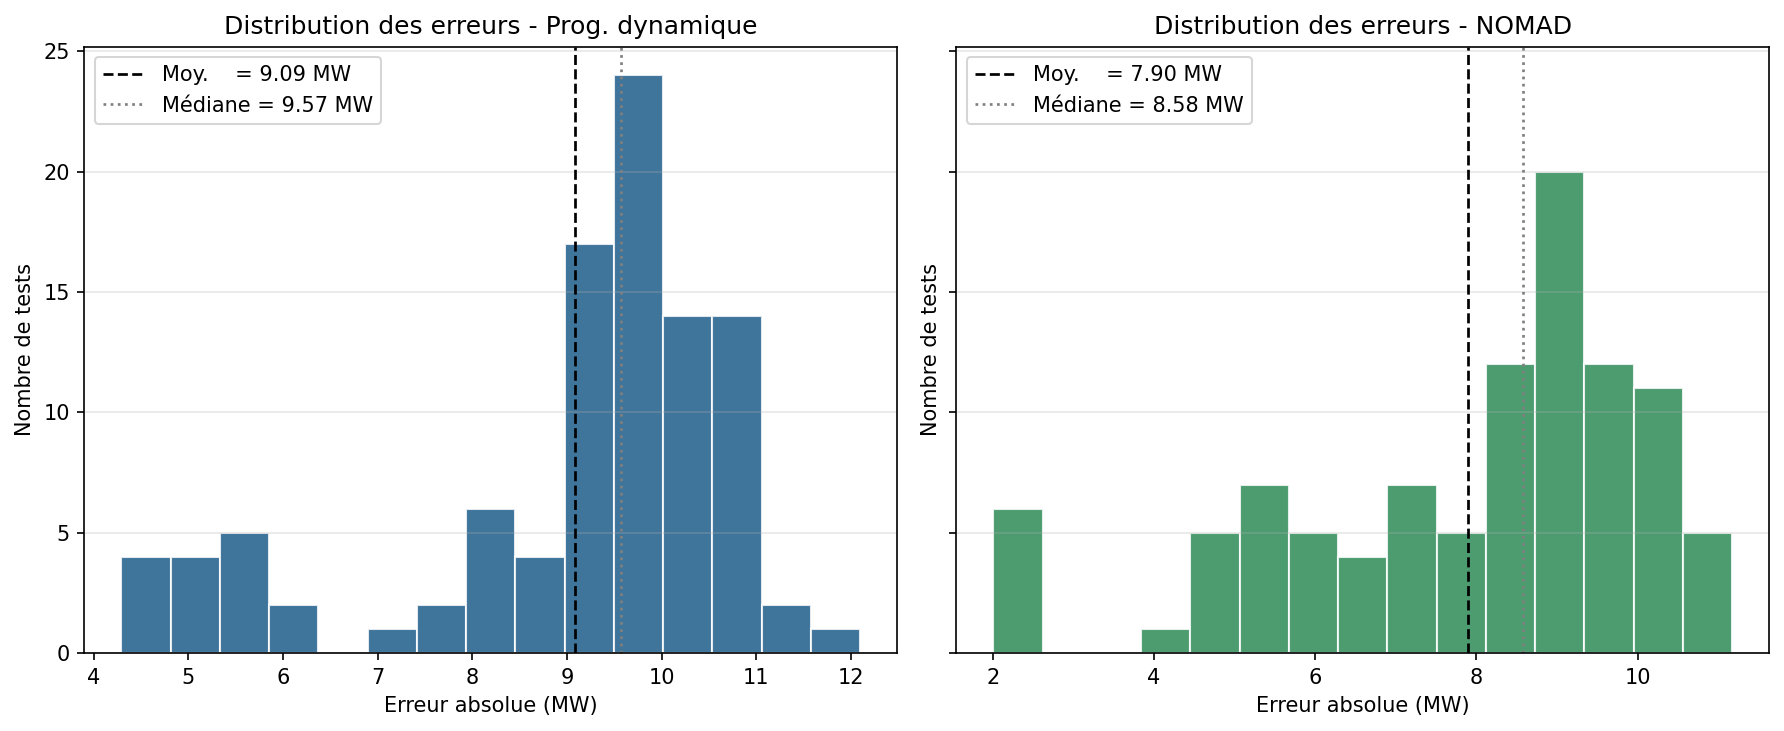
\includegraphics[width=0.85\textwidth]{graphiques_80/03_distribution_erreurs.png}
  \caption{Distribution des erreurs absolues - PD (gauche) et NOMAD (droite)}
  \label{fig:distrib_err}
\end{figure}

\begin{figure}[H]
  \centering
  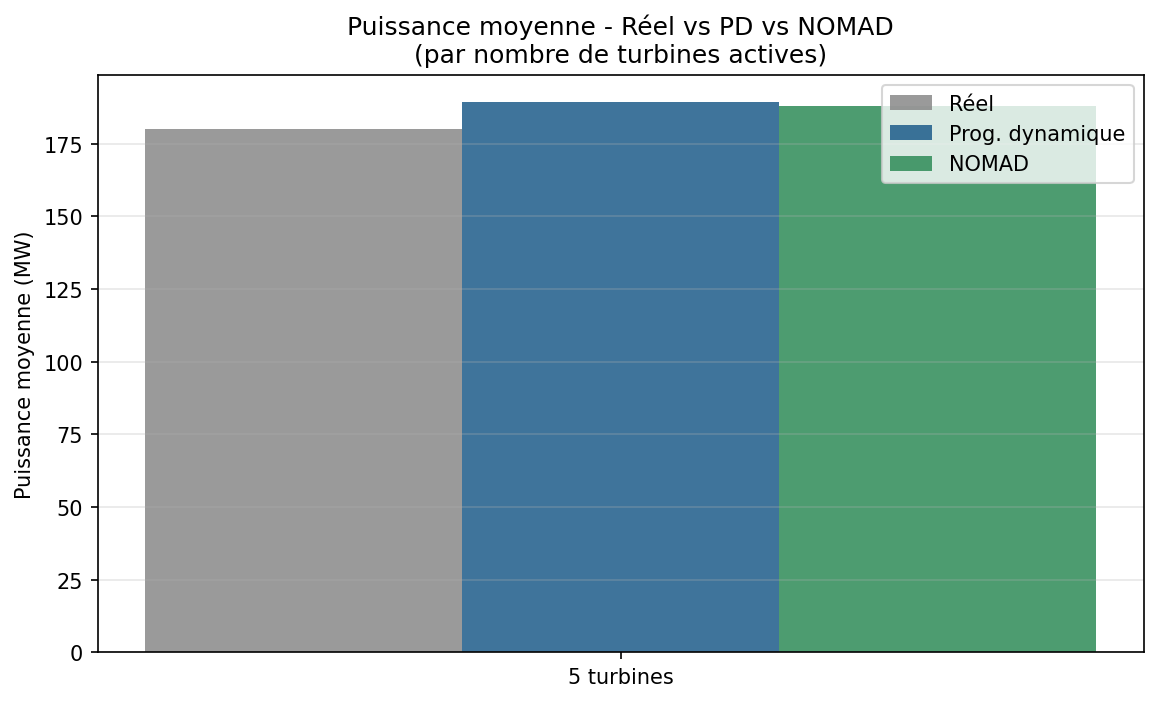
\includegraphics[width=0.5\textwidth]{graphiques_80/01_puissance_moyenne.png}
  \caption{Puissance moyenne produite - Réel vs PD vs NOMAD, par nombre de turbines actives}
  \label{fig:puissance_moy}
\end{figure}

\subsection{Temps de calcul}

La programmation dynamique est plusieurs ordres de grandeur plus rapide que NOMAD (0,033s contre 33,374s en moyenne). Ce résultat est attendu : la PD exploite la structure additive et séparable du problème et évite tout recalcul de sous-problèmes identiques.

À l'inverse, NOMAD fonctionne comme une boîte noire : chaque évaluation déclenche l'exécution d'un script qui lance un nouveau processus Python, puis un second processus pour analyser la réponse. Cette chaîne d'appels engendre une latence importante à chaque itération.

La réduction du nombre d'itérations de NOMAD à 80 a permis de diminuer significativement son temps de calcul, sans impact notable sur la qualité des solutions obtenues.

\begin{figure}[H]
  \centering

  \begin{minipage}{0.48\textwidth}
    \centering
    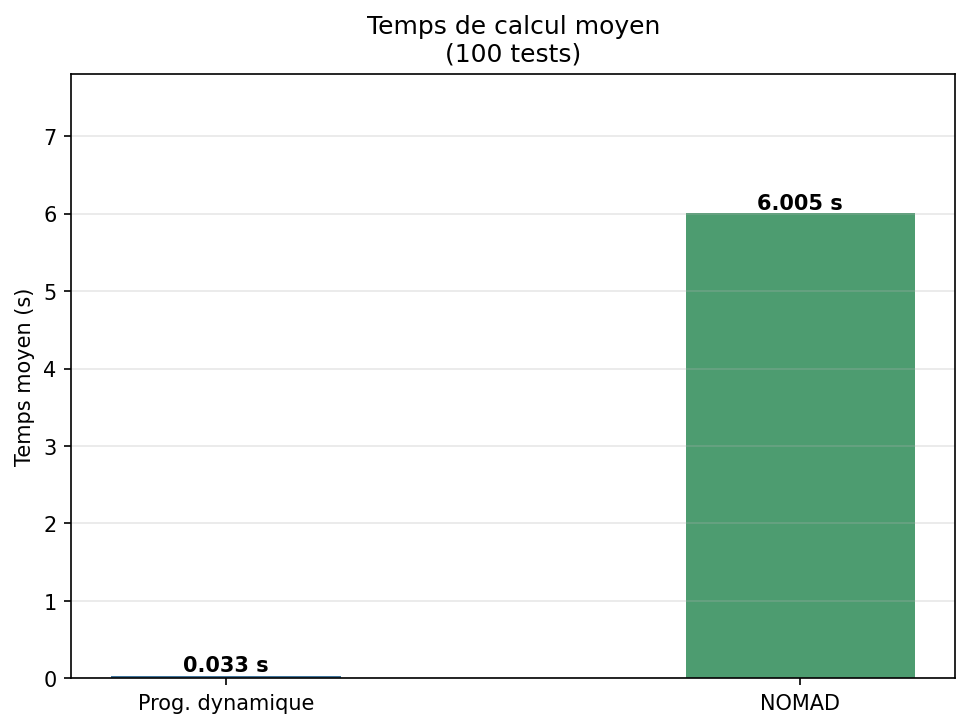
\includegraphics[width=\textwidth]{graphiques_80/05_5_temps_calcul.png}
    \caption*{(a) 80 itérations}
  \end{minipage}
  \hfill
  \begin{minipage}{0.48\textwidth}
    \centering
    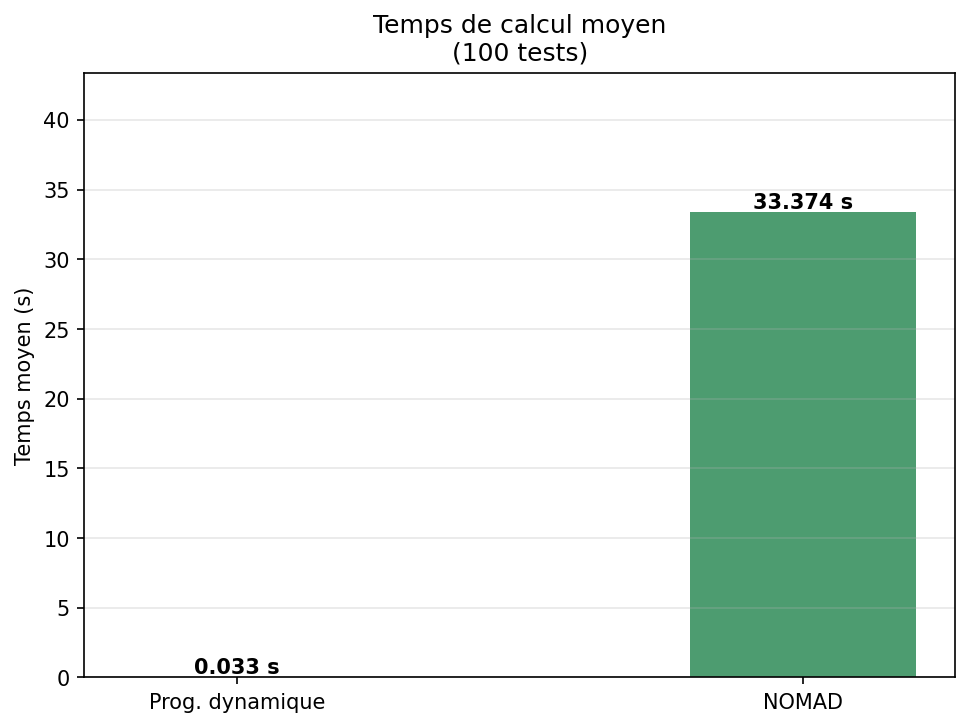
\includegraphics[width=\textwidth]{graphiques_max/05_5_temps_calcul.png}
    \caption*{(b) Itérations maximales}
  \end{minipage}

  \caption{Temps de calcul - PD vs NOMAD, global}
  \label{fig:temps_comparaison}
\end{figure}

\subsection{Nombre d'itérations}

Le nombre d'évaluations de la boîte noire varie selon la complexité du problème (nombre de turbines actives et débit total). NOMAD s'arrête lorsque le maillage devient trop fin pour améliorer la solution, ce qui correspond typiquement à quelques centaines d'évaluations pour ce problème de dimension 4.
Pour accélérer l'optimisation, nous avons réduit le nombre d'itérations à 80, soit 20\% du nombre maximal. Cela permet d'atteindre plus de 99\% de la précision maximale, ce qui est suffisant pour obtenir une solution de qualité comparable à celle de la PD, tout en réduisant significativement le temps de calcul (6 s contre 33 s en moyenne).
\begin{figure}[H]
  \centering

  \begin{minipage}{0.48\textwidth}
    \centering
    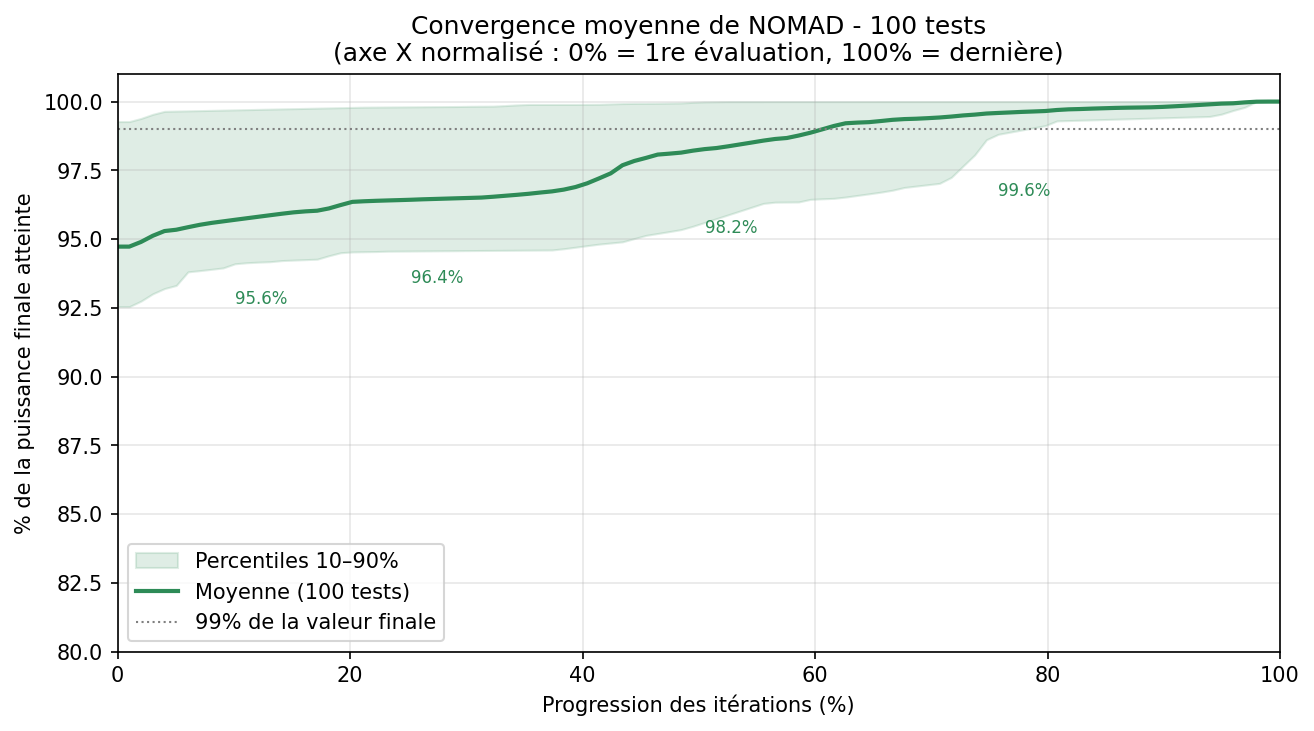
\includegraphics[width=\textwidth]{graphiques_80/08_convergence_moyenne.png}
    \caption*{(a) 80 itérations}
  \end{minipage}
  \hfill
  \begin{minipage}{0.48\textwidth}
    \centering
    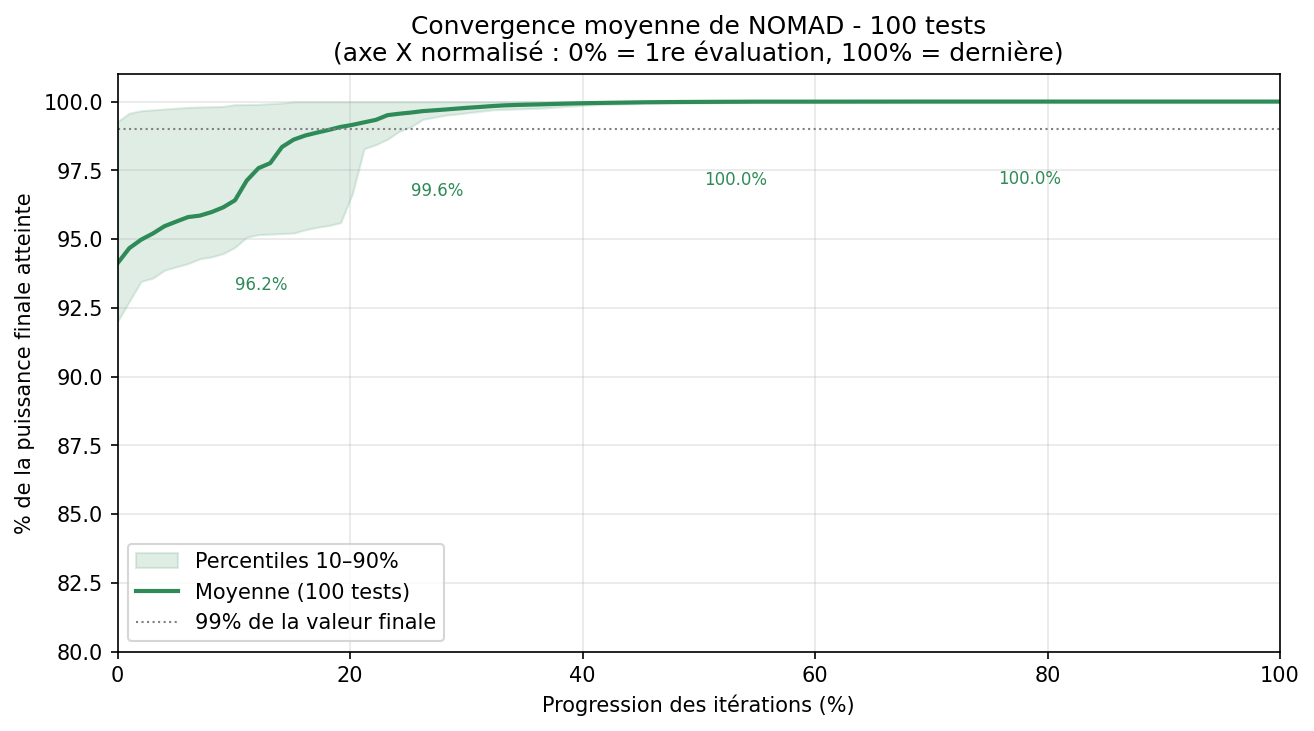
\includegraphics[width=\textwidth]{graphiques_max/08_convergence_moyenne.png}
    \caption*{(b) Itérations maximales}
  \end{minipage}

  \caption{Courbe de convergence moyenne de NOMAD sur 100 tests (axe X normalisé en \%)}
  \label{fig:temps_comparaison_convergence}
\end{figure}


\begin{figure}[H]
  \centering

  \begin{minipage}{0.48\textwidth}
    \centering
    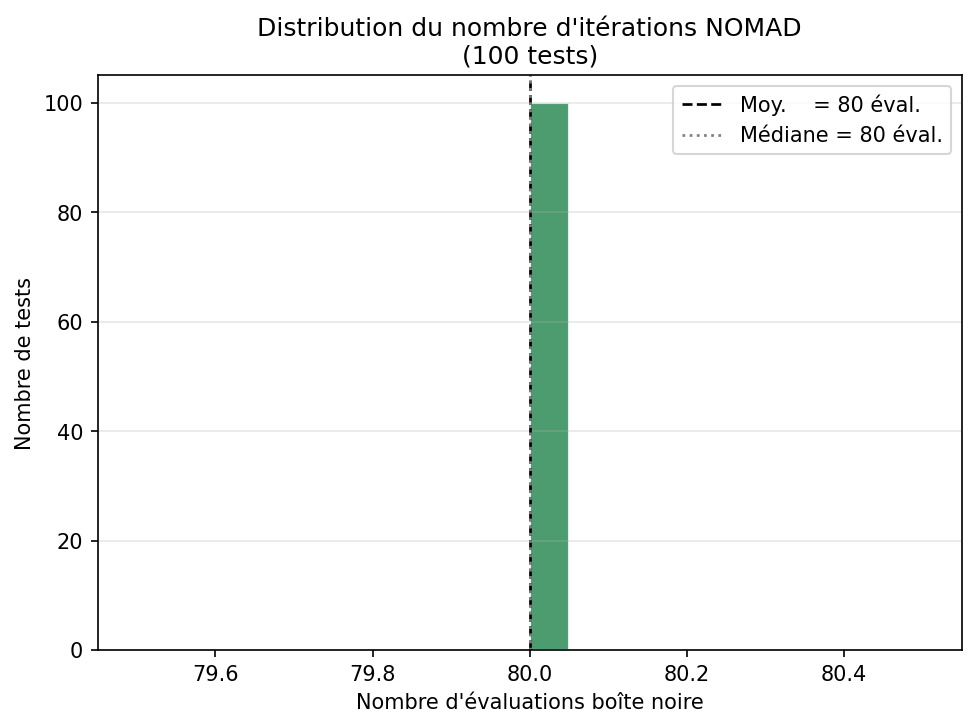
\includegraphics[width=\textwidth]{graphiques_80/04_5_iterations_nomad.png}
    \caption*{(a) 80 itérations}
  \end{minipage}
  \hfill
  \begin{minipage}{0.48\textwidth}
    \centering
    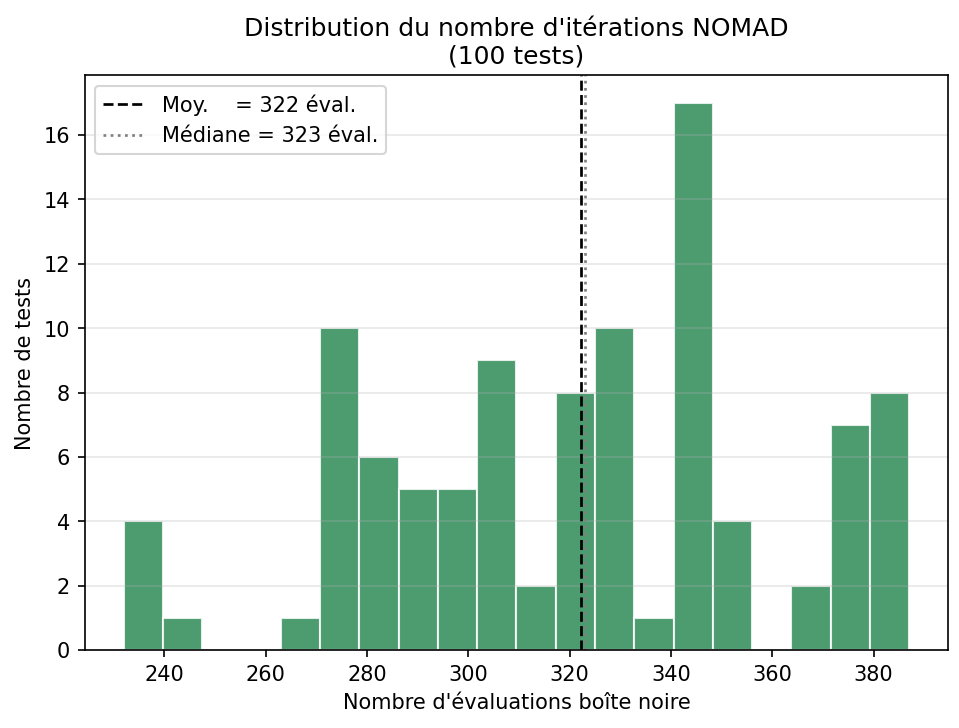
\includegraphics[width=\textwidth]{graphiques_max/04_5_iterations_nomad.png}
    \caption*{(b) Itérations maximales}
  \end{minipage}

  \caption{Nombre d'itérations (évaluations boîte noire) - distribution}
  \label{fig:distribution_iter}
\end{figure}


\subsection{Hypothèses}

En plus des hypothèses de la partie 1 (données fiables, validité des modèles poly33 hors des zones de données), l'optimisation boîte noire requiert les hypothèses supplémentaires suivantes. La dernière turbine est calculée par différence, ce qui suppose que la contrainte de débit total est satisfaite exactement après arrondi au palier de 5 m$^3$/s. De plus, l'algorithme NOMAD est utilisé comme un optimiseur de type local : la solution obtenue dépend du point de départ et du déroulement de la recherche, sans garantie d'atteindre la meilleure solution possible.

\subsection{Difficultés rencontrées}

L'intégration de NOMAD dans l'interface Flask a nécessité de résoudre plusieurs problèmes pratiques : la gestion des espaces dans le chemin de l'exécutable Python (résolue par un script \texttt{bb.bat} intermédiaire), le format exact du fichier \texttt{param.txt} requis par NOMAD 3.9, et le parsing de la sortie texte de NOMAD pour en extraire la meilleure solution et le nombre d'itérations.

% Conclusion
\chapter{Conclusion et travaux futurs}

Ce projet a permis de comparer deux approches d'optimisation complémentaires pour le problème de répartition optimale du débit dans une centrale hydroélectrique. La programmation dynamique offre une garantie d'optimalité et des temps de calcul très faibles, au prix d'une connaissance explicite des fonctions de production. L'optimisation boîte noire avec NOMAD est plus flexible - elle ne requiert pas de modèle analytique, mais est significativement plus lente et ne garantit pas l'optimalité.

Pour ce problème spécifique, les deux méthodes convergent vers des solutions de qualité, ce qui valide à la fois la qualité des modèles poly33 établis en partie 1 et la pertinence de la programmation dynamique comme méthode de référence.

Les travaux futurs pourraient inclure l'amélioration de l'interface graphique (avec par exemple, l’ajout du nombre d’itérations maximum), et l'exploration d'autres optimiseurs boîte noire pour comparer leurs performances avec NOMAD sur ce problème.

% ── Bibliographie ──────────────────────────────────────────
\printbibliography[heading=bibintoc, title={Bibliographie}]

\chapter{Annexe}
\section{Interfaces Projet 2}

\begin{figure}[H]
  \centering
   \includegraphics[width=1\textwidth]{figures/affichage2.png}
  \caption{Interface de test du projet 2}
  \label{fig:t2}
\end{figure}

\section{Validation des 100 premières lignes}
\begin{figure}[H]
  \centering
   \includegraphics[width=0.9\textwidth]{figures/validation4.png}
  \caption{Validation des 100 premières lignes avec 8100 itérations}
  \label{fig:t2}
\end{figure}

\begin{figure}[H]
  \centering
   \includegraphics[width=0.9\textwidth]{figures/validation3.png}
  \caption{Validation des 100 premières lignes avec 160 itérations}
  \label{fig:t2}
\end{figure}


\begin{figure}[H]
  \centering
   \includegraphics[width=0.9\textwidth]{figures/validation2.png}
  \caption{Validation des 100 premières lignes avec 80 itérations}
  \label{fig:t2}
\end{figure}

\section{Code du projet}
Fourni dans un fichier zip avec le rapport.

\end{document}

